\documentclass[conference]{IEEEtran}
\IEEEoverridecommandlockouts
% The preceding line is only needed to identify funding in the first footnote. If that is unneeded, please comment it out.
\usepackage[style=ieee, backend=biber]{biblatex}
\addbibresource{references.bib}
\addbibresource{ai_citations.bib}
\addbibresource{prerak.bib}
\usepackage{amsmath,amssymb,amsfonts}
\usepackage{algorithmic}
\usepackage{graphicx}
\usepackage{textcomp}
\usepackage{xcolor}
\def\BibTeX{{\rm B\kern-.05em{\sc i\kern-.025em b}\kern-.08em
    T\kern-.1667em\lower.7ex\hbox{E}\kern-.125emX}}
\begin{document}

\title{Human-Centered Intelligent Robots: A Literature Review\\
% \thanks{Identify applicable funding agency here. If none, delete this.}
}

\author{\IEEEauthorblockN{1\textsuperscript{st} Srijan Prasad Joshi}
\IEEEauthorblockA{\textit{Dept.\ of Computer Science} \\
\textit{Ramapo College of New Jersey}\\
Mahwah, United States of America \\
sjoshi3@ramapo.edu}
\and
\IEEEauthorblockN{2\textsuperscript{nd} Prerak Pandey}
\IEEEauthorblockA{\textit{Dept.\ of Computer Science} \\
\textit{Ramapo College of New Jersey}\\
Mahwah, United States of America \\
ppandey@ramapo.edu}
}

\maketitle

\begin{abstract}
Intelligent robots are becoming more and more mainstream. Tools such as Google voice assistant, becoming an integral part of many people's lives. As such, human-centered intelligent robot has become an important research field that spans across all fields in robotics such as intelligent control and path navigation. In this paper, we present the recent achievements of human-centered robotics and analyze the contemporary academic literature of this field. Furthermore, we look at the issues we had in the past, demonstrate why the recent approaches solved them, and discuss what the challenges that contemporary research are tying to solve in this field.
\end{abstract}

\begin{IEEEkeywords}
Human-centered robots, anthropomorphism, pattern recognition, computer vision, natural language processing, path planning, past issues, cloud based computing, computer hardware, intelligent control, navigation
\end{IEEEkeywords}

\section{Introduction}
Humanoid robots are very popular in science fiction. There are many movies such as the terminator where the robots are almost identical to humans. In the past two decade big progress has been made to make robots increasingly human. Compared to traditional robots such as industrial robots, human-centered robots require completely different performance measurement requirements\autocite{zinn2004new}. In this paper, we will present the various driver of this anthropomorphic development in robotics and delve into the literature that analyzes the contemporary research in them. We would be looking at how the advancements in pattern recognition predicate the rapid expansion of robotics logic. We would be looking at the important subfields of pattern recognition itself and present the relevant scientific literature surrounding each of those topics. We would also be presenting how progress in computer hardware is contributing to a large part to subsequent advancement in intelligent robotics technologies. We would then delve deep into why could computing is engendering all areas of computer science and in turn, robotics. We also look into the literature behind human-robot interaction and key in on the main application categories of this subfield. After we have present the status quo of research in all these fields, we present the current challenges in all these fields that the current research is trying to solve.

\section{Pattern Recognition}
The human brain has the capability to recognize various patterns to function. As such, we would want an anthropomorphic robot to use mimic this useful ability. In the past decade much progress has been made in this area of robotics given the rapid expanse of artificial intelligence. One main impetus for progress in pattern recognition is the rise of GPU accelerated machine learning techniques. One popular technique on the rise for pattern recognition is reinforcement learning where an agent uses many types of reinforcement learning which tries to maximize some sort of reward function for the agent. This sort of approach utilities mathematical models that uses. One common type of machine learning model used in robotics is the artificial neural network. However, though these have been proved to be very useful and though their distributed nature is similar to natural neural networks, their name itself is misleading because they have flaws like being brittle, inefficient, and myopic\autocite{Watson2019}. Though there are many projects that have used artificial neural networks to achieve very anthropomorphic results. One such project is famous alpha go project that used artificial neural networks to create an AI that beat Lee Sedol in a 6 game match against alpha go\autocite{silver2017mastering}. In that project, the neural network was initially trained using human game datasets and was then later trained using dataset of its own games\autocite{silver2017mastering}. Another project that was inspired from this project was a table tennis playing robot by \textcite{lin2020}. In that project, \textcite{lin2020} used Deep Neural Networks to handle parameters such as air resistance, the magnus effect, etc., and trained the said network using real life game simulations.

\subsection{Computer Vision}
One of the key driving factors of intelligent robots is the progress that we have made in computer vision in the past decade. Computer vision has been expanded into the vast area of field ranging from recording raw data into the extraction of image pattern and information interpretation\autocite{patel2012machine}. Most of the tasks in computer vision are related to observing input scenes and getting the necessary information from them. ``Computer vision works by using an algorithm and optical sensors to stimulate human visualization to automatically extract valuable information from an object''\autocite{wiley2018computer}. This field has been studied from many different perspectives and combines ideas from digital image processing, pattern recognition, machine learning, computer graphics, and human neurology. 

During the 1990s, there was not much progress made in this field. However, ever since \textcite{krizhevsky2012imagenet} published their paper on Alexnet and demonstrated their groundbreaking result on image classification using CNNs and GPU accelerated deep learning, there has been a boom in the future papers utilizing such tools. Robots now are capable of performing various forms of vision tasks that they were previously unable to perform. One famous modern application is in unmanned vehicles where the vehicle is able to navigate around its environments simply with the usage of visual data. Another is medical image processing where machine help medical professionals get information about patients from visual data. This boom in computer vision is so significant it even leads \textcite{pratt2015cambrian} to call it the possible ``robotics Cambrian explosion'' because this phenomenon of robotic achieving vision is just like the era when there was an exponential increase in evolutionary diversity largely caused by the natural creatures gaining vision. 


\subsection{Natural Language Processing}
Another area of artificial intelligence that is engendering anthropomorphic robots is the area of natural language processing. We as human beings have the most complex systems of utilizing natural sounds among any living creatures. We can form several different patterns and use sounds in complex ways to convey and understand information. As such, we would expect humanoid robots to be capable of handling such languages. The area of natural language processing is a branch of artificial intelligence that deals with the interaction between machines and humans using the natural language. This field just like computer vision has grown very big. In recent years we see exemplary tools such as Google translate and home assistant that have been made possible thorough natural language processing. According to \textcite{hirschberg2015advances} the main reasons for this are (i) increase in computing power (ii) availability of large amounts of linguistic data (iii) success of machine learning (iv) richer understanding of the structure of human language and its deployments in social contexts. The big progress done in this subfield are in machine translation (translating one language to another), spoken dialog systems and conversational agents (agents generating and interpreting human voice; e.g. Google assistant, Apple's Siri) and machine reading (the ability to interpret human written texts)\autocite{hirschberg2015advances}.

\section{Computer Hardware}
Moore’s law states that the number of transistors on a microprocessor chip will double every two years or so -- which has generally meant that the chip's performance will too\autocite{waldrop2016chips}. This has generally been true for the past several decades although  it is now encountering some fundamental physical limits. Semiconductor comanies are now manufacturing transistors on chips that are on a scale of 14 nanometers\autocite{pratt2015cambrian}. This small scale approach is reaching physical limit because of how close these transistor sizes are getting to the atomic level\autocite{waldrop2016chips}.

Furthermore, the usage of GPU accelerated has greatly expedited the speed that algorithms can run on. GPU or Graphics Processing Units made by NVIDIA or AMD were originally designed to be components in graphics subsystems. However, in the two few decades machine learning algorithms have greatly benefited from this hardware. Given the multi-threaded nature of GPUs, they act as the optimal option to perform matrix operations on\autocite{steinkraus2005using}. These matrix operations are at the heart of many machine learning algorithms. Fox example, the gradient descent algorithm in an artificial neural network could be thought of as a collection of matrix multiplications\autocite{krizhevsky2012imagenet}. The results that we are seeing from these new machine learning algorithms would have not been possible with the traditional single threaded CPU because executing single sequential instructions instead of multiple parallel instruction is much slower. 

Also, not just the improvement in computational speed, but even the readily available semiconductors are a large cause for the development of modern robotics. It is much cheaper to get the necessary tools required to build a robot in 2021 than it was ten or twenty years ago. This has significantly contributed to the increase research works in intelligent robots.

\section{Cloud Based Computing}
\subsection{Introduction to System Development of a Humanoid Robot}
As portrayed in the importance of emergence in the development of humanoid, artificially intelligent robots, it has always been desirable in the field, due to the complexity present in their research, to use the best platforms and tools to improve and develop algorithms that allow the code and tools to be reused to decrease the developmental effort required in the programming of these humanoid robot systems. A major roadblock in using these tools is the ability and time required to integrate these tools with existing systems and the incompatibility amongst the various software and tools used, as identified in the article by Martinez, Garcia-Haro, Monje, and Balaguer on the development of tools and applications for humanoid robots\autocite{1martinezdevelopment}. As defined by Bakken in 2001, in the robotics field, the main software environment that provides intercommunication and integration of tools is the middleware. This special kind of program was defined by Bakken as ``a class of software technologies designed to help to manage the complexity and heterogeneity inherent in distributed systems. It is defined as a layer of software above the operating system but below the application program that provides a common programming abstraction across a distributed system.''\autocite{2bakken2001middleware}

\subsection{Cloud computing in Humanoid Robot Development and Cloud Robotics}
\subsubsection{Introduction}
The term "cloud robotics" was coined in 2010 by James Kuffner, then at Carnegie Mellon University. The concept can be viewed as robots that are wirelessly linked to, and rely on, one or more computers in a remote location to support or facilitate certain aspects of its operation, i.e. where not all of the computation power, software, or memory is integrated into the robot\autocite{3bogue2017cloud}. The exploration of cloud computing and its use in cloud robotics is a topic surfacing to interest in recent years, however, research on the idea of using a "remote brain" on a robot has carried out from as early as the 1990s, when Masayuki Inaba, professor at the University of Tokyo explored this concept of remote brains, which he termed himself and this involved physically separating the robotic hardware from high-level reasoning software in a remote computer as quoted from Inaba in 1993 \autocite{3bogue2017cloud}. Now, cloud robotics technology seeks to build on that concept by exploiting the inexpensive computing power and massive data storage capacity of cloud computing systems, combined with the ubiquitous net connectivity available currently\autocite{3bogue2017cloud}. Below is a figure of the cloud configuration of a leading Cloud Robotics company, RoboEarth\autocite{13wan2016cloud}.

\begin{figure}[h]
    \centerline{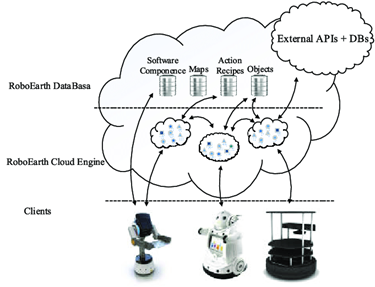
\includegraphics[width=0.5\textwidth]{prerak_images/Picture1.png}}
    \caption{Figure showing cloud architecture for cloud robotics\autocite{13wan2016cloud}}
\label{prerakfig1}
\end{figure}

\subsubsection{Application and Developments of Cloud Computing on Humanoid Robots}
With the advancement in data storage, management, and manipulation through cloud computing, The ability to access huge data sets, massive computational power and all manner of APIs is of potential benefit to most classes of robots, as mentioned by Bogue in his journal on cloud robotics\autocite{3bogue2017cloud}. The application of cloud technologies has been proposed for the development of many mobile/autonomous robotic vehicles, surgical, household, and military robots. It has also been recognized that humanoid robots are prime applicants for cloud computing. The aim of many humanoids is to interact with humans through speech but natural language processing, i.e. the ability to understand the subtleties of context and meaning, poses a huge technological challenge and requires massive and power-hungry signal processing, something that cannot realistically be incorporated into a small humanoid robot. Accordingly, in most cases at present, a humanoid robot's speech patterns are still limited to a range of stilted, programmed responses that are usually based on trigger words and pre-set behavior\autocite{3bogue2017cloud}. These limitations are changing – and are on the verge of mitigation with the application of cloud computing.

\subsubsection{Implementation}
In October 2019, CloudMinds Technology Inc., one of the world's leading cloud robot and services company, demoed their humanoid service robots at the Mobile World Congress in Los Angeles, which is described as the first humanoid robot in the United States to use cloud-based AI and 5G connectivity. The service robot, named XR-1, implements a cloud-first approach to robotics and artificial intelligence development, as according to CloudMinds, for service robots to be truly useful, they need artificial intelligence running on the cloud accessible over 5G networks, and to ensure minimal latency\autocite{4demaitre_demaitre_2020}.

\begin{figure}[h]
    \centerline{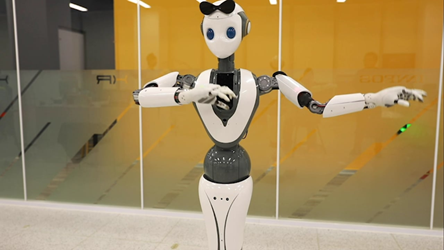
\includegraphics[width=0.5\textwidth]{prerak_images/Picture2.png}}
    \caption{XR-1 Humanoid Robot at MWC Los Angeles\autocite{4demaitre_demaitre_2020}}
\label{prerakfig2}
\end{figure}

As another example, Ericsson, the Swedish telecoms giant, is looking into the cloud robotic possibilities presented by the upcoming 5G network. In addition to faster speeds, 5G can meet the demands of modern and evolving technologies such as the Internet of Things, allowing for higher numbers of concurrently connected devices, lower latency, and new levels of reliability, making it suitable for cloud computing. Manufacturing, agriculture, factories, and health care are among the possible applications listed by Ericsson. Mobile cloud robot prototypes have already been demonstrated in a simulated space, transferring materials between work-cells and a warehouse\ref{prerakfig3}. A laser rangefinder was used for navigation, and a webcam was used for pattern recognition. The trials began with a learning process, during which the laser rangefinder produced a map of the working area that was later used by the robot for localization\autocite{3bogue2017cloud}

\begin{figure}[h]
    \centerline{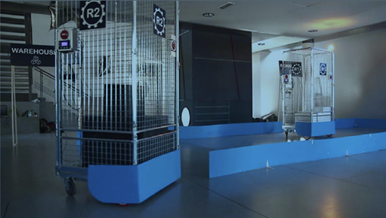
\includegraphics[width=0.5\textwidth]{prerak_images/Picture3.png}}
    \caption{Experimental Setup of the Simulated Space, Ericsson\autocite{3bogue2017cloud}}
\label{prerakfig3}
\end{figure}

\subsubsection{Limitations}
Though cloud computing can provide many advantages that humanoid robots can benefit from, however, there are also limitations to its use in different circumstances. Some of these limitations to cloud computation in development of humanoid robots are listed below:
\begin{itemize}
\item{} Controlling a robot's motion, which is heavily reliant on (real-time) sensors and controller feedback, cannot benefit greatly from cloud computing as latency might cause implications in time sensitive tasks. For example, if a humanoid robots are used in explosive defusal tasks, the latency of a fraction of a second to determine whether task is successful or not.
\item{} Too much reliability of the humanoid robot on the cloud could result in the robot malfunctioning or unable to function due to a fault in the cloud network.
\item{} Heavier reliance on cloud computing also exposes the robot system to remote security threats. A significant cloud sharing environment for a robot is often a target for malwares, brute force attacks and virtual machine attacks.
\end{itemize}
Cloud robotics technology is rapidly maturing, as shown by the advances and applications described above. More than two decades have passed since Inaba's seminal publication on the use of a “remote brain”, during which time technical advancements have accelerated at an unparalleled pace. Developments in several fields of artificial intelligence, especially pattern recognition and natural language processing, will invariably improve the capabilities of cloud robots. Even though cloud robotics is still in its beginnings, it is not hard to anticipate that in the future, almost all robots will be connected to cloud-based computer systems.
\subsection{Navigation}
\subsubsection{Motion in Humanoid Robots}
Existing humanoid robots are currently planned for a variety of purposes and applications. Each humanoid robot is built with unique characteristics, skills, and equipment, all of which affect the overall structure, expense, and complexity of production. Humanoid robots in most examples use bipedal locomotion and have a humanoid appearance. Existing humanoid robots have a variety of capabilities, making them one of the most versatile robots in a variety of applications such as education, assisting, entertainment and tasks physically difficult and risky for human such as rescues.

As stated by Saeed Saeedvand and authors in their scholarly journal on humanoid robot development, most of the humanoid robots are generally able to walk bipedally in different environments with different abilities, with more recent developments including the ability of humanoid robots to walk stably on flat grounds, grass, and also uneven environments\autocite{5saeedvand2019comprehensive}. Humanoid robots with a bipedal locomotion system offer different advantages over wheeled robots. Bipedal robots are more suitable for navigating in a complex workplace, and they are more adaptable\autocite{6silva2007historical}\autocite{6al2014modeling}. Due to the difference in the task and abilities of a robot, navigation is based on specifically designed parts for the robot, which is challenging and requires a comprehensive study of the different parts and functionalities that make up the humanoid robot. Thus, navigation is based on both the hardware design and the software implementation used during the development of the robot. The software and hardware developmental aspects of a humanoid robot are further studied below.

\subsubsection{Hardware architecture and configuration for Navigation}
The mechanical design of humanoid robots is the most important aspect of their creation. The architecture of humanoid robots' mechanical structure and kinematics has been influenced by human structure and kinematics.
Each joint of a humanoid robot has some parameters that determine the state of a physical system, such as the degrees of freedom (DOF). The total number of independent displacements or aspects of motion is equal to the number of robot’s DOF. A humanoid robot includes torso, hip, head, neck, two arms, hands, legs, and feet, and each joint in a humanoid robot can be rotated in three orthogonal axes in maximum as roll, pitch, and yaw\autocite{5saeedvand2019comprehensive}.Figure \ref{prerakfig4} shows a labelled diagram of an XR-1 humanoid robot model. With higher number of degrees of freedom in multiple joints, its navigational and locomotive development is very complex.

\begin{figure}[h]
    \centerline{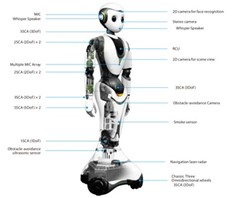
\includegraphics[width=0.5\textwidth]{prerak_images/Picture4.jpg}}
    \caption{Figure displaying different DOFs in XR-1 from CloudMinds\autocite{4demaitre_demaitre_2020}}
\label{prerakfig4}
\end{figure}

The figure below provides specification of the number of DOFs of some well known adult-sized and child-sized  humanoid robots

\begin{figure}[h]
    \centerline{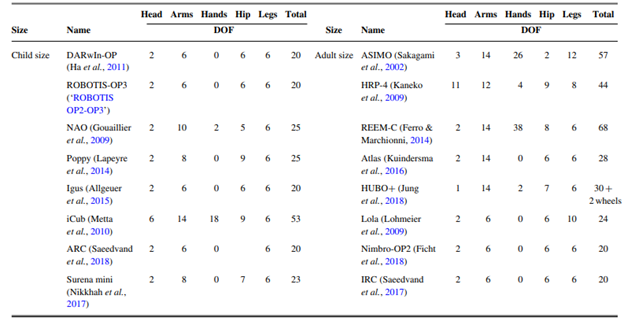
\includegraphics[width=0.5\textwidth]{prerak_images/Picture7.png}}
    \caption{Figure showing specifications of the number of DOFs of some well-known humanioid robot models}
\label{prerakfig5}
\end{figure}

There are different hardware components required to allow movement of a humanoid robot arm, with respect to the tasks required to be done and the features the robot system will provide, they are as follows:

\subsubsection{Actuators for Humanoid Robots}
Different types of joint types have been established in the last century, based on the importance of the control system on humanoid robot locomotion and its relationship to the robot's joints and corresponding actuators (e.g., linear, revolute, sliding, or spherical). In several structures, spherical joints are one of the most common joint types. Hydraulic, pneumatic, or linear electric actuators are often used in spherical joints. The majority of revolute joints are electrically driven by stepper motors or servo motors, despite the fact that hydraulic and pneumatic rotary joints are common. However, spherical joints have multiple degrees of freedom, thus is more complex to control.

\subsubsection{Processing Units for Humanoid Robot}
 Humanoid robots have one or more processing units in addition to their mechanical structure. In general, the electronic components used in humanoid robots are chosen based on the target application, such as whether the robot is autonomous or remote, the robot's missions, the cost of relevant components, and so on. Commercial controlling boards are used widely in addition to hand-made controlling boards. Raspberry Pi boards\autocite{7mejias2017easy} , ARM-based boards \autocite{9almubarak2017design}, compatible Arduino boards \autocite{8al2012development}, or off-board computing controls\autocite{10khokar2015implementation} are all examples of this.

 \subsubsection{Sensors for Humanoid Robot}
There are several experiments that have been conducted in order to improve robot interactions in the environment and achieve powerful sensors. Nonetheless, robot sensing systems are still restricted, and achieving a human-like sensing system can seem impractical\autocite{5saeedvand2019comprehensive}. Camera sensors, pressure sensors, laser scanners, and inertial measuring units (IMUs) are all popular sensors used in humanoid robots.

The IMU is the most significant sensor in humanoid robots because of their bipedal configuration. An IMU is a sensor that uses a combination of accelerometers, gyroscopes, and magnetometers to calculate and record a body's specific force, angular rate, and the magnetic field surrounding it. On humanoid robots, the IMU usually is attached to the upper body and measures the angles and angular velocities against the ground in sagittal and frontal planes\autocite{11cho2011online}. The produced data from IMUs firstly are arranged through filtering algorithms, then walk engines are used for development\autocite{5saeedvand2019comprehensive}.

\subsubsection{Power Supply for Humanoid Robot}
Portable and rechargeable battery packs are typically used to power a bipedal humanoid robot. Portable generators are also used in some situations. Rechargeable batteries come in a variety of shapes and sizes, and they are often used in mobile robots. Li-PO batteries are the most popular battery type on humanoid robots (lithium-polymer) with advantages of higher energy density, safe performance, high discharge rate, and withstanding high frequency charging cycles\autocite{5saeedvand2019comprehensive}.

    Figure \ref{prerakfig6} below provides specification of the hardware configurations of some well-known humanoid robot models categorized as child-sized and Figure\autocite{7mejias2017easy} provides specifications for well know adult-sized humanoid robot models\autocite{5saeedvand2019comprehensive}:

\begin{figure}[h]
    \centerline{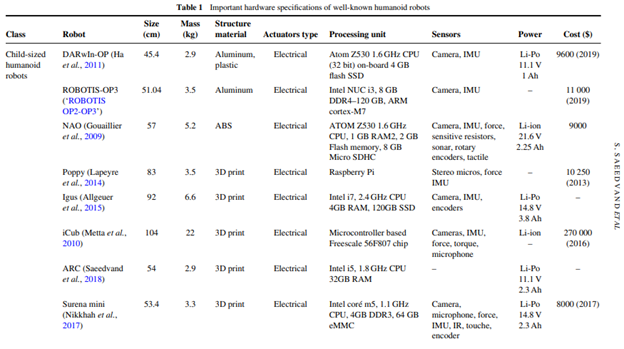
\includegraphics[width=0.5\textwidth]{prerak_images/Picture8.png}}
    \caption{Hardware Specifications of Child-sized humanoid robots}
\label{prerakfig6}
\end{figure}


\begin{figure}[h]
    \centerline{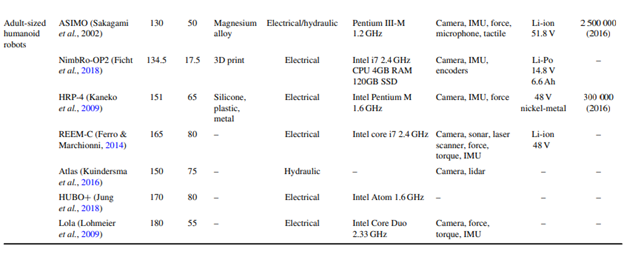
\includegraphics[width=0.5\textwidth]{prerak_images/Picture9.png}}
    \caption{Hardware Specifications of Adult-sized humanoid robots}
\label{prerakfig7}
\end{figure}

\subsection{Software Architecture and Configuration for navigation}
The Robot Operating System (ROS) was created to address the issue of diversity and to provide unification as well as a faster implementation process\autocite{5saeedvand2019comprehensive}. ROS is a collection of software libraries and resources that enable researchers to create robot applications.
The general software aspects to allow movement and navigation, most common in use in humanoid robots, are as follows:

\subsubsection{vision}
The camera is one of the most important sensors for perception. Real-time robot vision algorithms are also needed to extract information from the captured images. Monocular and stereo vision devices are used for humanoid robots. It is well accepted that a monocular vision system cannot provide accurate information about the environment because of its linearity, which creates a motion pattern without complete observations. A stereo vision system consists of two cameras usually equipped with a controller module for stereo processing. Using the stereo vision system can enable the robot to measure the distance of objects, to detect the floor, and to generate a path for walking around obstacles\autocite{5saeedvand2019comprehensive}.

\subsubsection{Walk (locomotion) control}
A humanoid robot should be able to walk omnidirectionally and at various speeds on various surfaces. The aim of omnidirectional walking is to provide a robot with dependable, flexible, and dynamic locomotion. However, omnidirectional walk regulation can be difficult in certain situations and harsh conditions. For example, in disaster rescue scenarios, robots must be able to walk around obstacles and along narrow paths.
To create the stability required in the system to enable humanoid robot movement and navigation, the primary criterion to be processed in the robot’s center of mass (COM) and center of pressure (COP) and is stable if these centers fall in the vertical column created by the area of the base\autocite{12wang2012optimizing}. The secondary criterion is the quasi-dynamic walking, based on the concept of zero moment point, which is a point on the ground where the results of the reaction forces on the ground act.

\subsubsection{Behavior control}
Due to the wide range of applications, path planning and navigation in autonomous humanoid robots is a promising research area. In humanoid robots, behavior control primarily consists of path planning, which is the process of determining the best sequence of actions that will enable the robot to walk from its starting point to its destination without colliding with obstacles. Several strong artificial intelligence techniques have been proposed to solve route planning and navigation of humanoid robots in complex environments, there is yet to be a fully suitable solution.

\section{Human-Robot Interactions}
\begin{figure}[h]
    \centerline{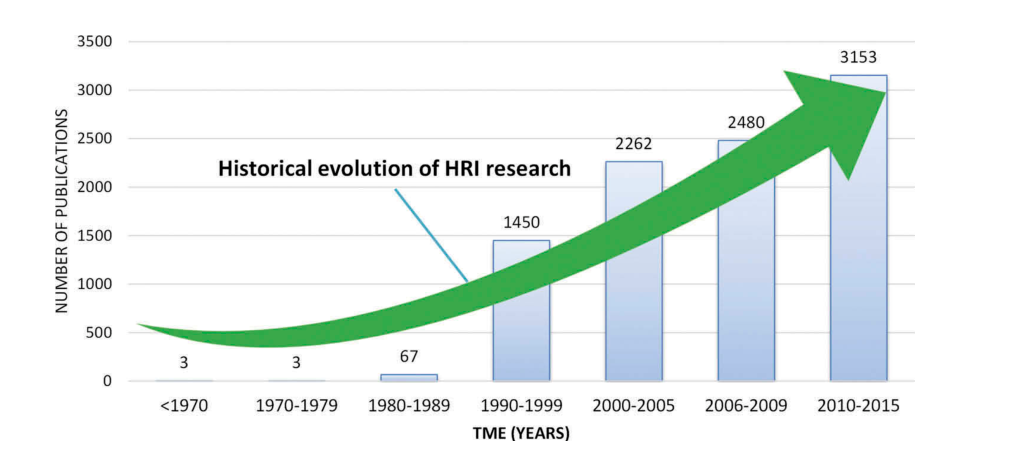
\includegraphics[width=0.5\textwidth]{images/evolution_of_hri.png}}
    \caption{Figure showing the increase in the publications related to HRI from 1960 - 2015. Figure gotten from\autocite{tsarouchi2016human}}
\label{fig1}
\end{figure}

\begin{figure}[h]
    \centerline{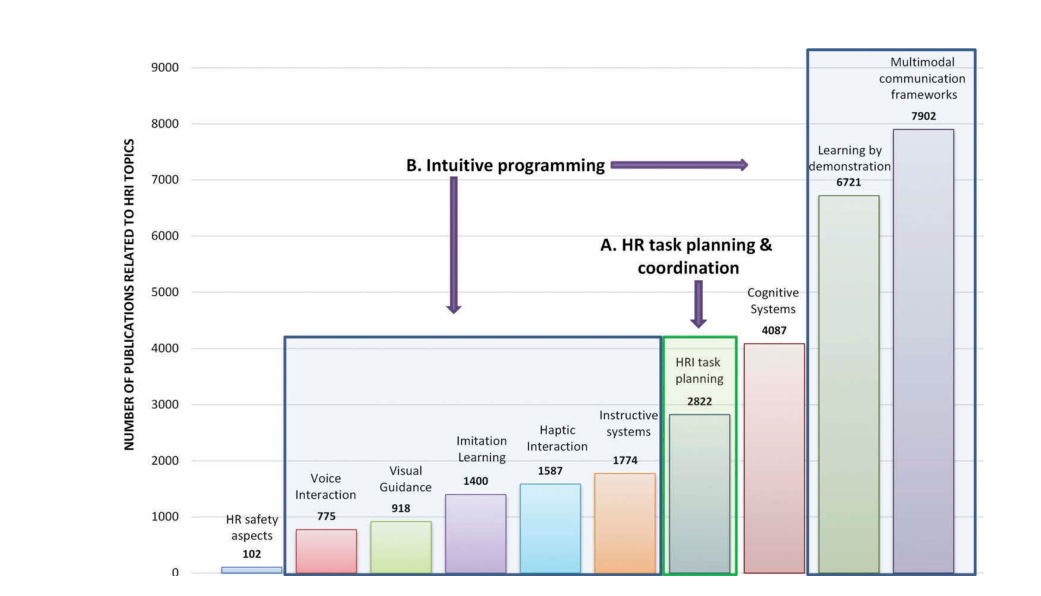
\includegraphics[width=0.5\textwidth]{images/hri_total_number_of_publication.png}}
    \caption{Figure showing the total number of publications from 1970-2015 within per aspect of HRI. The two most dominating subfields are ``Learning by demonstration'' and ``Multimodal communication frameworks''. Figure gotten from \autocite{tsarouchi2016human}}
\label{fig2}
\end{figure}

Human-robot interaction is an expanding field with hundreds of publications being published each year by many different professional societies (as shown in figure \ref{fig1}). \textcite{sheridan2016human} states that HRI can be roughly divided into four areas of application: Human supervisory control of robots in performance of routine tasks; Remote control of space, airborne, terrestrial, and undersea vehicles for non-routine tasks in hazardous or inaccessible environments, automated vehicles in which a human is a passenger, and Human–robot social interaction. 
\begin{itemize}
\item \textbf{Human supervisory control of robots in performance of routine tasks:} This area deals with handling parts on manufacturing assembly lines and the delivery of packages, components, mail, and medicines in warehouses, offices and hospitals\autocite{sheridan2016human}. Human operators are required to supervise the use of such machines and it is an important area in intelligent robotics. There are still much research being Safety is a big concern in this subfield.
\item \textbf{Remove control of Vehicles:} Robots being needed to operate in hazardous areas and not endanger humans to such places were one of the primary motivators of early robotics development.Much progress has been made in remote control of unmanned spacecraft, undersea robotic vehicles, and unmanned aerial vehicles. Human factors research continues to be needed for improving and simplifying display and control interfaces\autocite{sheridan2016human}. There are promising developments in using robotic avatars for surveillance, search and rescue for police work, border patrol, firefighting and rescue, and military operations, with many human factor issues for display and control and mental workload\autocite{sheridan2016human}.
\item \textbf{Automated Vehicles With Human Passenger:} One famous new technology that arouses much excitement is the new driverless vehicles. ``As is well known, recently Google has produced a self-driven car, demonstrated successfully on California freeway''\autocite{sheridan2016human}. This area has certainly gotten more and more successful these past ten years. However, one large safety issue in this field is the human driver not staying alert and take over should the automation fail. We already have minimized the error rate to to less that 0.1 percent. However, this is still considered too large for this technology to be utilized in the mainstream.
\item \textbf{Human-Robot Social Interactions:} Robots functioning in social situations and becoming more anthropomorphic is a big part of human-robot interactions. We want humanoid robots to be able to demonstrate the same social abilities as humans and participate in social situations competently. The Sophia bot developed by Hanson AI is a famous example that is capable of mimicking human facial expressions and speech patterns.
\end{itemize}


\section{Major Contemporary Challenges}
\begin{figure}
    \centerline{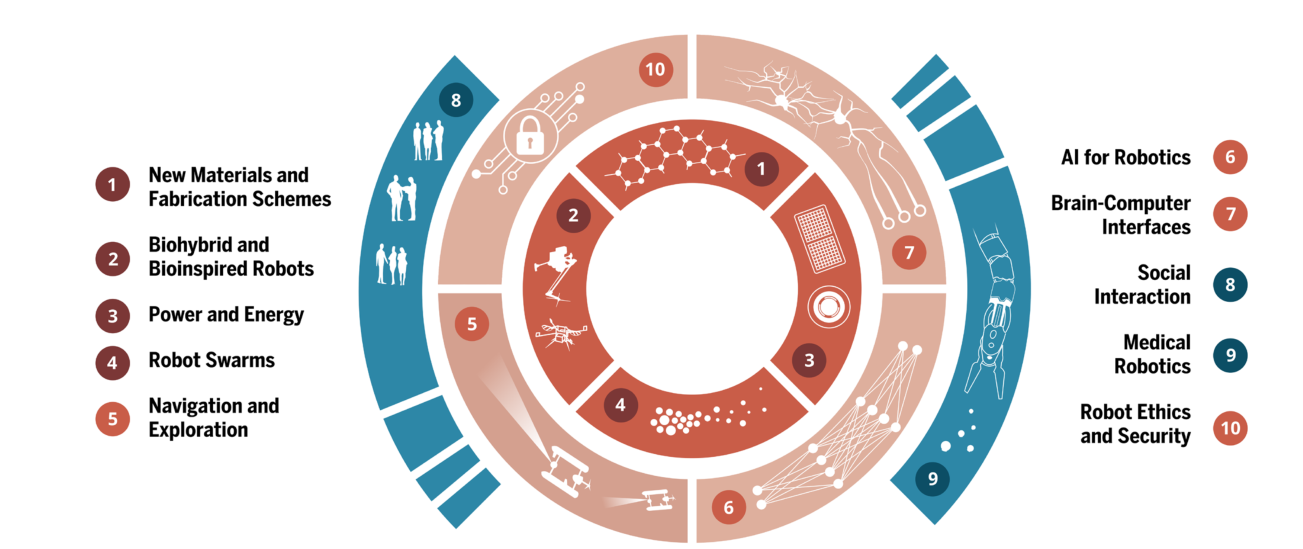
\includegraphics[width=0.5\textwidth]{images/grand_challenges.png}}
    \caption{Figure showcasing the challenges big challenges to modern robotics. Figure gotten from\autocite{yang2018grand}}
\label{fig3}
\end{figure}

In the paper "The grand challenges of Science Robotics", the authors \textcite{yang2018grand} mention the following as the biggest challenges to future robotics for the next 5 - 10 years. They can easily be interpolated to human-centered robots as well.
\begin{itemize}
\item \textbf{Robot swarms:} Emergence is one of the most interesting observations we see in our natural environment. Robots swarms replicate natural emergence and allow simpler, less expensive, modular robotic units to be reconfigured into a team. Robot networks integrated with our infrastructure have tremendous potential for solving the most pressing problems facing human civilization. 
\item \textbf{Brain-computer interfaces:} A brain-computer interface forms a direct connection between the human brain and machine. ``Direct use of brain activity to control a computer or external device without the mediation of the peripheral, somatomotor nervous system has major applications in enabling paralyzed patients to communicate and control robotic prosthetics and in rehabilitation for restoring neural function''\autocite{yang2018grand}. However, in this field there are challenges like sensing and acquiring acquisition being cumbersome, data processing and dealing with artifacts of non cerebral origin, particularly for wearable approaches, and finding out if BCI will ever outperform simpler techniques like eye tracking or muscle based devices.
\item \textbf{Social interaction:}Because humans are so adept at recognizing and interpreting social behavior, we often underestimate the complexity of the challenge that this represents for a robot. Social interaction is a major challenge for robotics in part because the perceptual demands are so significant. Social cues—such as gaze direction, facial expressions, or vocal intonation—are often extremely detailed. There are many details to consider for robot can appropriately evaluate social these cues and act accordingly. This is certainly a big challenge in this field.
\item \textbf{New Materials and their fabrication schemes:} Gears, motors, and mechanical actuators have always been the use in many robotic projects. However, newer generation of robots are exploring ``new materials including artificial muscles, compliant materials for soft robots, and emerging advanced manufacturing and assembly strategies''\autocite{yang2018grand} These new genre of materials are power efficient, multi functional, compliant, and autonomous in ways that are similar to biological organisms. ``However, most demonstrations using new materials and fabrication strategies have been “one-offs” and must still overcome basic hurdles to achieve wide-scale adoption''\autocite{yang2018grand}. 
\item \textbf{Bioinspired and biohybrid robots:} Bioinspired robotics in our context means the  use of fundamental biological principles that are translated into engineering design rules for creating robots. If the biological understanding results in the direct use of biological material to design synthetic machines, then our context refers to this as a biohybrid robot. For biohybrid and bioinspired robots, actuation and energy remain major bottlenecks compared with performance seen in animals. As bioinspired robots venture beyond the laboratory, models of real-world, unstructured environments will be required, but none can yet adequately represent our complex, dynamic world
\item \textbf{Navigation and exploration:} Though we have achieve a lot in term of navigation, there are still challenges in this area. One is that robots struggle to operate in environments that are unmapped and when the environment's nature is not understood\autocite{yang2018grand}. For navigation, the grand challenge is to handle failures and being able to adapt, learn, and recover. For exploration, it is developing the innate abilities to make and recognize new discoveries.
\item \textbf{Fundamental aspects of artificial intelligence for robotics:} The advent of deep learning methods resulted in remarkable levels of object recognition accuracy (61) using hierarchical pattern recognition that retained information coherence at each level of the hierarchy. However, we still are not anywhere near reaching the intelligence that we see in humans.
\item \textbf{Ethics and security:} With increasing levels of autonomy and humanrobot interaction, there needs to be careful consideration of potential regulatory, ethical, and legal barriers and the context of how robots are deployed. Technologies like STARRA are projected become more and more commonplace in the workforce. As such, there are many ethical question that comes up in regards to utilizing these machines as we progress to the future. The field of ethics and security is an important field for robotics and AI.
\end{itemize}

\section{Conclusion}
Many robots will be put into application in our daily lives in the future; some, maybe many, will look and act like humans, but portraying and utilizing humanoid properties that provides a technical advantage over their more utilitarian counterparts is an implementation that is more complex to develop and maintain. With the growing size and significance of implementations and platforms particular to the development of humanoid robots, these complexities rise to create concerns in the performance of these robots, and even though complete solutions to fully mitigate these complexities do not and will not ideally exist, extensive growing research in the field almost promises a future where humans coexist with assisting humanoid robots.

\printbibliography{}
\end{document}
